\documentclass[20pt,letterpaper]{article}
\usepackage{fullpage}
\usepackage[top=1.5cm, bottom=1.5cm, left=1.5cm, right=1.5cm]{geometry}
\usepackage{amsmath,amsthm,amsfonts,amssymb,amscd}
\usepackage{lastpage}
\usepackage{enumerate}
\usepackage{fancyhdr}
\usepackage{mathrsfs}
\usepackage{xcolor}
\usepackage{graphicx}
\usepackage{listings}
\usepackage{hyperref}

\hypersetup{%
  colorlinks=true,
  linkcolor=blue,
  linkbordercolor={0 0 1}
}
 
\renewcommand\lstlistingname{step}
\renewcommand\lstlistlistingname{Algorithms}
\def\lstlistingautorefname{Alg.}

\lstdefinestyle{Python}{
    language        = C++,
    frame           = lines, 
    basicstyle      = \footnotesize,
    keywordstyle    = \color{blue},
    stringstyle     = \color{green},
    commentstyle    = \color{red}\ttfamily
}

\setlength{\parindent}{0.0in}
\setlength{\parskip}{0.05in}

% Edit these as appropriate
\newcommand\course{CS 372}
\newcommand\hwnumber{1}                  % <-- homework number
\newcommand\NetIDa{NAVEEN}           % <-- NetID of person #1
\newcommand\NetIDb{1601CS28}           % <-- NetID of person #2 (Comment this line out for problem sets)

\pagestyle{fancyplain}
\headheight 35pt
\lhead{\NetIDa}
\lhead{\NetIDa\\\NetIDb}                 % <-- Comment this line out for problem sets (make sure you are person #1)
\chead{\textbf{\Large Graphics Assignment No:- \hwnumber}}
\rhead{\course \\ \today}
\lfoot{}
\cfoot{}
\rfoot{\small\thepage}
\headsep 1.5em

\begin{document}

\section*{1. Assignment description}

  OpenGL, short for \textbf{Open Graphics Library,} is an application programming interface (API) designed for rendering 2D and 3D graphics. It provides a common set of commands that can be used to manage graphics in different applications and on multiple platforms.


\section*{2. Procedure}

\begin{enumerate}

    \item Install Xcode, which is a suite of software development tools for Mac OS X
    \item The steps to installing and running OpenGL on the Mac OS X are few because OpenGL is integrated into the operating system:
    \lstset{caption={Install GLEW}}
    \lstset{label={lst:alg1}}
     \begin{lstlisting}[style = Python]
      Using brew install glew
      Install GLEW by going to http://glew.sourceforge.net/index.html 
      and following instructions
    \end{lstlisting}

  \item
  \textbf{Using OpenGL and GLUT in source}
    \lstset{caption={ Link framework with openGL project}}   
  \begin{lstlisting}
  \end{lstlisting}
    Start Xcode and choose File → New project from the drop-down menu; create a new Cocoa Application by choosing it from the menu. Deselect main.m, and instead add your source codes in the Other Sources folder. From the top-left drop-down menu in the window, click on Add →Existing Frameworks, and add three frameworks,Cocoa frameworks, OpenGL framework and GLUT framework,both from the Frameworks folder. (These frameworks are located in / System/ Library/Frameworks/. )
   \item 
    \textbf{Finally in your source include the files as needed}
 \lstset{caption={ C++ include header file}}   
\begin{lstlisting}
   1.#include <OpenGL/gl.h>
   2.#include <OpenGL/glu.h>
   3.#include <GLUT/glut.h>
\end{lstlisting}
   \item
    draw line using  function glVertex2i,glEnd,glFlush,glBegin,
    glClear,etc .
\end{enumerate}
\section*{3. Result}
    \textbf {\huge Line}
     \begin{figure}[!h]
    \centering
    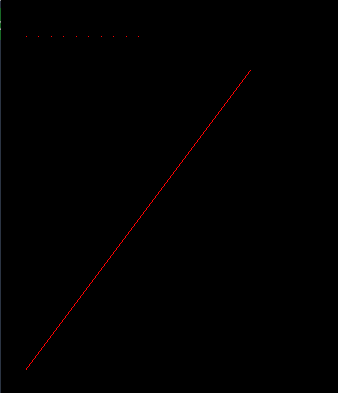
\includegraphics[width=0.5\linewidth]{openGL_line.jpg}
    \caption{Using OpenGL(C++ library) line drawing}
    \end{figure}

\section*{4. Python}
  \textbf{ Drawing of circle , line ,rectangle,ellipse,polyline using OpenCv}
  \begin{figure}[!h]
    \centering
    \includegraphics[width=0.5\linewidth]{square_circle_opencv.jpg}
    \caption{Using OpenCv(Python library) line,circle and rectangle etc. }
    \end{figure}
\end{document}
